\documentclass[homework]{IEEEtran}
\IEEEoverridecommandlockouts
% The preceding line is only needed to identify funding in the first footnote. If that is unneeded, please comment it out.
\usepackage{cite}
\usepackage{CJKutf8}
\usepackage{indentfirst}
\usepackage{amsmath,amssymb,amsfonts}
\usepackage{algorithmic}
\usepackage{graphicx}
\usepackage{textcomp}
\usepackage{xcolor}
\usepackage[justification=centering]{caption}
\setlength{\parindent}{2em}
\def\BibTeX{{\rm B\kern-.05em{\sc i\kern-.025em b}\kern-.08em
    T\kern-.1667em\lower.7ex\hbox{E}\kern-.125emX}}
\begin{document}

\title{Homework of Pattern classification\\
{\footnotesize \textsuperscript{*}Name: Xue Yuan  | Student number: 202228015926034}
}

\author{}
\maketitle

\begin{abstract}
This document is about the first homework for Pattern classification by \LaTeX.
\end{abstract}

\section{Question 1}
\begin{CJK}{UTF8}{gkai}
    请描述最小错误率贝叶斯决策的计算步骤(包含已知条件以及求解任务);给出一种两类情形下的最小错误率贝叶斯决策规则。\par
    \begin{enumerate}[已知条件:]
		\item 先验概率  $$ P\left(\omega_i\right), \quad \sum_{i=1}^c P\left(\omega_i\right)=1 $$
		\item 概率密度函数(条件概率) $P\left(\omega_i\vert\\x\right)$
    	\end{enumerate}\par
    求解任务: \par如果观测到一个样本x,那么应该将其分到哪一类才最合理呢?\par
    两类情形下的最小错误率贝叶斯决策规则:\par
        if $p\left(\mathbf{x} \mid \omega_1\right) P\left(\omega_1\right)>p\left(\mathbf{x} \mid \omega_2\right) P\left(\omega_2\right)$, then $\mathbf{x} \in \omega_1$; otherwise $\mathbf{x} \in \omega_2$
\end{CJK}
\section{Question 2}
\begin{CJK}{UTF8}{gkai}
    请描述最小风险贝叶斯决策的计算步骤(包含已知条件以及求解任务);给出一种两类情形下的最小风险贝叶斯决策规则。\par
    \begin{enumerate}[已知条件:]
		\item 先验概率  $$ P\left(\omega_i\right), \quad \sum_{i=1}^c P\left(\omega_i\right)=1 $$
		\item 概率密度函数(条件概率) $P\left(\omega_i\vert\\x\right)$
		\item 决策空间包含a个决策$\alpha_i$,i=1,2,...,a
		\item 损失函数$P\left(\lambda_i\vert\omega_j\right)$,表示当类别为$\omega_j$所采取的决
        策$\alpha_i$所引起的损失,简记为$\lambda_{ij}$。
    	\end{enumerate}\par
求解任务:\par如果观测到一个样本x,那么应该将其分到哪一类其风险最小?\par
两类情形下的最小风险贝叶斯决策规则:
        $$R\left(\alpha_i \mid \mathbf{x}\right)=E\left[\lambda\left(\alpha_i \mid \omega_j\right)\right]=\sum_{j=1}^c \lambda\left(\alpha_i \mid \omega_j\right) P\left(\omega_j \mid \mathbf{x}\right)$$
         $i=1,2, \ldots, a$;  And if $R\left(\alpha_1 \mid \mathbf{x}\right) <R\left(\alpha_2 \mid \mathbf{x}\right)$, then $\alpha = \alpha_1$; otherwise $\alpha = \alpha_2$
\end{CJK}

\section{Question 3}
\begin{CJK}{UTF8}{gkai}
    对于 c 类问题,假定各类条件概率密度函数均为多元正态分布。在最小错误
    率贝叶斯决策的框架下,请写出其判别函数;请分别指出在什么情况下可以
    获得最小距离分类器,在什么情况下可以得到线性判别函数。\par
最小错误率贝叶斯决策框架下的判别函数:
		\begin{equation}
            \begin{aligned}
            g_i(\mathbf{x}) &=\ln \left(p\left(\mathbf{x} \mid \omega_i\right)\right)+\ln \left(P\left(\omega_i\right)\right) \\
            &=-\frac{1}{2}\left(\mathbf{x}-\boldsymbol{\mu}_i\right)^T \boldsymbol{\Sigma}_i^{-1}\left(\mathbf{x}-\boldsymbol{\mu}_i\right)\\
            &-\frac{d}{2} \ln (2 \pi)-\frac{1}{2} \ln \left(\left|\boldsymbol{\Sigma}_i\right|\right)+\ln \left(P\left(\omega_i\right)\right)\\
            &\left(i=1,2, \ldots, a\right)
            \end{aligned} \nonumber
        \end{equation} \par
最小距离分类器:\par
         当样本的协方差矩阵相等且等于一常数,即$\sum_i$=$\sigma^2\I$, i=1,2,...,c。且先验概率相等即: $P\left(\omega_i\right)$=$P\left(\omega_j\right)$,此时,判别函数可进一步简单化为: $$g_i(\mathbf{x})=-\frac{1}{2 \sigma^2}\left\|\mathbf{x}-\boldsymbol{\mu}_i\right\|_2^2$$ \par
         此时,要对样本x进行分类, 只需要计算x到各类均值向的欧氏距离平方, 然后将归于距离最短的一类:$$\arg \min _{i=1,2, \ldots, c}\left\|\mathbf{x}-\boldsymbol{\mu}_i\right\|_2^2$$ \par 
         这样的分类器我们称最小距离分类器\par
    \begin{enumerate}[线性判别函数:]
        \item 与最小距离分类器的条件类似,当先验概率不相等即$P\left(\omega_i\right)$ $\neq$ $P\left(\omega_j\right)$时,判别函数$g_i(\mathbf{x})$可以写成:
        $$\begin{aligned}
            g_i(\mathbf{x}) &=-\frac{1}{2 \sigma^2}\left(\mathbf{x}-\boldsymbol{\mu}_i\right)^T\left(\mathbf{x}-\boldsymbol{\mu}_i\right)+\ln \left(P\left(\omega_i\right)\right) \\
            &=-\frac{1}{2 \sigma^2}\left(\mathbf{x}^T \mathbf{x}-2 \boldsymbol{\mu}_i^T \mathbf{x}+\boldsymbol{\mu}_i^T \boldsymbol{\mu}_i\right)+\ln \left(P\left(\omega_i\right)\right)
          \end{aligned}$$
        \item 由于每一类的判别函数均包含 $\mathbf{x}^T \mathbf{x}$, 与下标 $i$ 无关, 因此可以进一步简化为线性判别函数:
        $$
        \begin{aligned}
         g_i(\mathbf{x}) =\frac{1}{\sigma^2} \boldsymbol{\mu}_i^T \mathbf{x}-\frac{1}{2 \sigma^2} \boldsymbol{\mu}_i^T \boldsymbol{\mu}_i+\ln \left(P\left(\omega_i\right)\right) =\mathbf{w}_i^T \mathbf{x}+w_{i 0} \\
            \mathbf{w}_i=\frac{1}{\sigma^2} \boldsymbol{\mu}_i \qquad w_{i 0}=\ln \left(P\left(\omega_i\right)\right)-\frac{1}{2 \sigma^2} \boldsymbol{\mu}_i^T \boldsymbol{\mu}_i
        \end{aligned}$$
    \end{enumerate}
\end{CJK}

\section{Question 4}
\begin{CJK}{UTF8}{gkai}
    针对概率密度函数参数估计问题,请描述最大似然估计的计算步骤(包含已知条件以及求解任务)。 \par
    \begin{enumerate}[已知条件:]
		\item 假设每组样本都是从类条件概率具有形式$P\left(\\x\vert\omega_i\right)$的总体中独立重复抽取出来的
		\item 类条件概率函数$P\left(\\x\vert\omega_i\right)$具有未知参数$\theta$,参数$\theta$表征了总体X的一种或几种特征(如均值或方差等)
		\item 各类样本仅仅包含本类的分布信息,不同类别的参数$\theta$相互独立
    	\end{enumerate}
    求解任务: \par
        给定样本集$D=\left\{\\X_1,\\X_2,\dots,\\X_n\right\}$,要找到一个条件概率最大的参数$\theta$,即求:$$\arg \max_\theta P\left(D\vert\theta\right)$$
    \begin{enumerate}[计算步骤:]
        \item 从总体中独立重复的抽取样本得到样本集$D=\left\{\\X_1,\\X_2,\dots,\\X_n\right\}$
        \item 视每一次抽样为一个概率事件,那么,独立的获得n个样本的联合概率(称似然函数$l(\boldsymbol{\theta})$)为:
        $$
        l(\boldsymbol{\theta})=P(D \mid \boldsymbol{\theta})=P\left(\mathbf{x}_1, \mathbf{x}_2 \ldots, \mathbf{x}_n \mid \boldsymbol{\theta}\right)=\prod_{i=1}^n p\left(\mathbf{x}_i \mid \boldsymbol{\theta}\right)
        $$
        它描述了在不同参数取值下取得当前样本的可能性。为了计算方便,我们有时也会采用对数形式下的似然函数$H(\boldsymbol{\theta})$:
        $$
        H(\boldsymbol{\theta})=\ln (l(\boldsymbol{\theta}))=\ln \prod_{i=1}^n p\left(\mathbf{x}_i \mid \boldsymbol{\theta}\right)=\sum_{i=1}^n \ln \left(p\left(\mathbf{x}_i \mid \boldsymbol{\theta}\right)\right)
        $$
        \item 当我们从样本空间中选取到的参数$\hat\theta$,使得似然函数$l(\boldsymbol{\theta})$(或$H(\boldsymbol{\theta})$)取最大值时,我们便称
        $\hat\theta$为参数$\theta$的最大似然估计量
        \item 确定了似然函数以后,通过对似然函数求导(多维情况下求梯度),我们能够得到参数$\theta$的最大似然估计值
    \end{enumerate}
\end{CJK}

\section{Question 5}
\begin{CJK}{UTF8}{gkai}
    针对样本的类条件概率密度函数估计问题,请描述贝叶斯估计的计算步骤(包含已知条件以及求解任务)。 \par
    已知条件: \par
            贝叶斯估计与最大似然估计在整体上几乎一致,只是在待估参数的处理上存在差异。贝叶斯估计认为,待估参数是一个随机变量,而样$D$是固定的(一经取得),需要对待估参数的分布进行重点估计。\par
    \begin{enumerate}[求解任务:] \par
        \item 通过先验概率$p(\theta)$(没有掌握数据时,参数$\theta$的分布情况)和样本分布估计后验概率$P(\theta\vert\ D)$(掌握了一定量的数据后参数$\theta$的分布情况)
        \item 不断学习使得后验概率$P(\theta\vert\ D)$取最大
        \item 通过最大$P(\theta\vert\ D)$结合样本分布情况估计总体的概率分布$P\left( x \vert D \right)$
        \end{enumerate}\par
    \begin{enumerate}[计算步骤:]
        \item 由贝叶斯公式,后验概率$P(\theta\vert\ D)$可以表示为: $$
        P(\boldsymbol{\theta} \mid D)=\frac{P(D \mid \boldsymbol{\theta}) p(\boldsymbol{\theta})}{p(D)}
        $$
        \item 由全概率公式:$$
        p(D)=\int_{\boldsymbol{\theta}} p(D \mid \boldsymbol{\theta}) p(\boldsymbol{\theta}) d \boldsymbol{\theta}
        $$
        可以得到:$$
        P(D \mid \boldsymbol{\theta})=P\left(\mathbf{x}_1, \mathbf{x}_2 \ldots, \mathbf{x}_n \mid \boldsymbol{\theta}\right)=\prod_{i=1}^n p\left(\mathbf{x}_i \mid \boldsymbol{\theta}\right)
        $$
        \item 带入1)中,有贝叶斯参数估计中的后验概率密度函数:$$
        P(\boldsymbol{\theta} \mid D)=\frac{P(D \mid \boldsymbol{\theta}) p(\boldsymbol{\theta})}{
            \int_{\boldsymbol{\theta}} \prod_{i=1}^n p\left(\mathbf{x}_i \mid \boldsymbol{\theta}\right) p(\boldsymbol{\theta}) d \boldsymbol{\theta}}
            = \alpha\prod_{i=1}^n p\left(\mathbf{x}_i \mid \boldsymbol{\theta}\right) p(\theta)
        $$
        \item 考虑边际分部,可以得到:
        \begin{equation}
            \begin{aligned}
            P\left(x\vert D\right) &= \int_{\boldsymbol{\theta}} p\left(x,\theta\vert D\right) d \boldsymbol{\theta} \\
                &=\int_{\boldsymbol{\theta}} \frac{P(x,\boldsymbol{\theta},D)}{p(D)}d\boldsymbol{\theta} \\
                &=\int_{\boldsymbol{\theta}} \frac{p(x\vert{\theta,D})p\left(\theta,D\right)}{p(D)}d\boldsymbol{\theta}\\
                &=\int_{\boldsymbol{\theta}} p(x\vert{\theta,D})p\left(\theta\vert D\right)d\boldsymbol{\theta}\\
                &=\int_{\boldsymbol{\theta}} p(x\vert\theta)p\left(\theta\vert D\right)d\boldsymbol{\theta}
            \end{aligned}
            \nonumber
        \end{equation}
    \end{enumerate}\par
    考虑总体自身的分布情况,我们就完成了通过样本估计后验概率,再由后验概率估计总体概率分布的任务(Fig1展示了这一过程)。
\end{CJK}

\begin{figure}[htb]
    \centerline{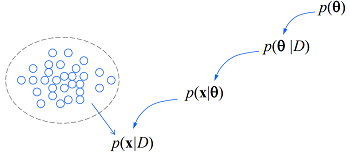
\includegraphics{Images/fig1.png}}
    \caption{Flowchart of the estimation process.}
    \label{fig}
\end{figure}
\section{Question 6}
\begin{CJK}{UTF8}{gkai}
    请指出最大似然估计和贝叶斯估计的不同之处? \par
    他们之间最大的差异在于对待估参数的认识:\par 
    最大似然估计认为,待估参数是存在的,同时,假定样本D是随机的。可以通过总体抽取出的样本,对待估参数进行准确估计。\par 
    贝叶斯估计则认为,参数是随机变量,而样本D 是固定的。由于样本是固定的,因此重点研究待估参数的分布。
\end{CJK}

\end{document}
